% =====================================================================
%  Presentación de TEG · Plantilla
%  Compilar con:  latexmk -xelatex presentacion.tex
%            o:   xelatex presentacion.tex (dos veces)
% =====================================================================
\documentclass[aspectratio=169,11pt]{beamer}
\usepackage[spanish,es-noshorthands,es-nodecimaldot]{babel}
\usepackage{amsmath,amssymb,mathtools}
\usetheme{TEG}            % opción: \usetheme[sinprogreso]{TEG}

\usepackage{tikz}
\usetikzlibrary{shapes.geometric, arrows.meta, positioning}
\usepackage{multirow}
\usepackage[backend=biber,style=numeric]{biblatex}
\addbibresource{references.bib}

% ---------------------------------------------------------------------
%  Datos de la portada
% ---------------------------------------------------------------------
\title{Predicci\'on probabil\'istica de resultados de partidos de f\'utbol}
\subtitle{mediante un sistema de rating din\'amico Glicko-2 con integraci\'on de factores deportivos, econ\'omicos y ambientales}
\author[Rub\'en Arellano]{Br. Rub\'en Alejandro Arellano Platt}
\grado{Licenciatura en Matemática}
\tutor{Profa. Maira Valera-L\'opez}
\institute{Escuela de Matemática\\Facultad de Ciencias · UCV}
\date{Caracas, 01 de Octubre de 2026}
\contacto{ruben.arellano@ciens.ucv.ve}

\logoizquierdo{
\includegraphics[height=13mm]{logos/ucv.png}}
\logoderecho{
\includegraphics[height=11mm]{logos/escuela-matematica.jpg}}

\begin{document}

% ---------------------------------------------------------------------
\begin{frame}[plain,noframenumbering]
  \titlepage
\end{frame}

\begin{frame}{Contenido}
  \scriptsize
  \tableofcontents[hideallsubsections]
\end{frame}

% =====================================================================
\section{Contexto y brecha}
% =====================================================================

% ---------- Slide 3: Antecedentes ----------
\begin{frame}{Antecedentes}{Rankings institucionales y sistemas de rating}
	\begin{columns}[T,onlytextwidth]
		\column{.48\textwidth}
		\tegetiqueta{Rankings institucionales}\par\vskip 2mm
		\footnotesize
		FIFA, UEFA, CONMEBOL, AFC, CONCACAF, IFFHS.
		\begin{itemize}
			\item Escalar determinista.
			\item Sin medida de incertidumbre.
			\item Empate como ausencia de se\~nal.
		\end{itemize}
		\column{.48\textwidth}
		\tegetiqueta{Sistemas de rating}\par\vskip 2mm
		\footnotesize
		Elo (1978) $\to$ Glicko (1995) $\to$ Glicko-2 (2022) $\to$ Shelopugin-Sirotkin (2023).
		\begin{itemize}
			\item Incertidumbre v\'ia $RD$.
			\item Empate como categor\'ia estoc\'astica.
			\item Sin covariables ex\'ogenas.
		\end{itemize}
	\end{columns}
	\vfill
	\secundario{\small Ninguno cubre los tres elementos: conteo, rating din\'amico y covariables.}
\end{frame}

% ---------- Slide 4: La brecha ----------
\begin{frame}[t]{Planteamiento del problema}{La brecha}
	\small
	\begin{itemize}
		\item Un modelo de conteo que derive probabilidades por resultado.
		\item Un rating din\'amico que actualice fuerza e incertidumbre de forma secuencial.
		\item Un mecanismo que incorpore covariables ex\'ogenas.
	\end{itemize}
	\vskip 1mm
	La brecha no es la ausencia individual de cada componente, sino su \textbf{falta de articulaci\'on} en un solo \textit{pipeline} que cubra las limitaciones del anterior.
\end{frame}

% ---------- Slide 5: Pregunta de investigación ----------
\begin{frame}[t]{Pregunta de investigación}
	\vfill
	\begin{alertblock}{}
		\centering
		\large
		\emph{¿C\'omo estimar probabil\'isticamente el resultado de un partido integrando informaci\'on deportiva, econ\'omica y ambiental, con actualizaci\'on secuencial y cuantificaci\'on de la incertidumbre sobre la fuerza de cada equipo?}
	\end{alertblock}
	\vfill
\end{frame}

% ---------- Slide 6: Objetivos ----------
\begin{frame}[shrink]{Objetivos}
	\footnotesize
	\begin{columns}[T,onlytextwidth]
		\column{.44\textwidth}
		\tegetiqueta{Objetivo general}\par\vskip 2mm
		Desarrollar un sistema en cascada para estimar probabil\'isticamente el resultado de partidos a partir de informaci\'on deportiva, econ\'omica y ambiental, con actualizaci\'on secuencial y cuantificaci\'on de la incertidumbre.
		\column{.52\textwidth}
		\tegetiqueta{Objetivos espec\'ificos}\par\vskip 2mm
		\begin{enumerate}
			\item Implementar el bloque de conteo que estima tasas de goles y deriva la probabilidad de empate.
			\item Construir el Glicko-2 modificado con calibraci\'on de la ventaja de local\'ia por liga.
			\item Dise\~nar el perceptr\'on multicapa que refina las probabilidades base con covariables.
			\item Evaluar con diez ejecuciones pareadas e inferencia mediante test $t$.
		\end{enumerate}
	\end{columns}
\end{frame}

% ---------- Slide 7: Arquitectura en cascada ----------
\begin{frame}{Arquitectura en cascada}
	\centering
	\resizebox{0.95\textwidth}{!}{%
	\begin{tikzpicture}[
		node distance=1.2cm and 1.8cm,
		block/.style={rectangle, draw=tegAcento, fill=tegGrisClaro,
			rounded corners, text width=2.4cm, align=center,
			minimum height=1.1cm, font=\small},
		arrow/.style={-{Stealth[length=3mm]}, thick, tegAcento},
		lbl/.style={font=\scriptsize, tegGris}
		]
		% Bloques
		\node[block] (skellam) {Skellam/LGBM};
		\node[block, right=of skellam] (g2a) {G2Av1513};
		\node[block, right=of g2a] (mlp) {MLP};
		
		% Entrada
		\node[left=of skellam, text width=1.8cm, align=center, font=\scriptsize] (input)
		{Goles hist\'oricos\\(rollings)};
		\draw[arrow] (input) -- (skellam);
		
		% Flechas
		\draw[arrow] (skellam) -- node[above,lbl]{$P_D^{(S)}$} (g2a);
		\draw[arrow] (g2a) -- node[above,lbl]{$(P_H,P_D,P_A)$} (mlp);
		
		% Covariables al MLP
		\node[above=0.8cm of mlp, text width=2.2cm, align=center, font=\scriptsize] (cov)
		{Covariables\\ex\'ogenas};
		\draw[arrow] (cov) -- (mlp);
		
		% Salida
		\node[right=of mlp, text width=1.6cm, align=center, font=\scriptsize] (output)
		{$(\tilde{P}_H,\tilde{P}_D,\tilde{P}_A)$};
		\draw[arrow] (mlp) -- (output);
		
		% R\'otulos inferiores
		\node[below=0.3cm of g2a, lbl] {actualizaci\'on secuencial};
		\node[below=0.3cm of mlp, lbl] {refinamiento no param\'etrico};
	\end{tikzpicture}}%
	\vfill
	\secundario{\small Cada bloque cubre una limitaci\'on del anterior.}
\end{frame}

% =====================================================================
\section{\textit{Pipeline} de datos}
% =====================================================================

% ---------- Slide 8: Diseño del pipeline ----------
\begin{frame}[t]{Pipeline de datos}{Seis etapas, de archivos crudos a datasets finales}
	\centering
	\resizebox{0.75\textwidth}{!}{%
		\begin{tikzpicture}[
			node distance=0.6cm and 0.7cm,
			etapa/.style={rectangle, draw=tegAcento, fill=tegGrisClaro,
				rounded corners, text width=2.4cm, align=center,
				minimum height=1.2cm, font=\small},
			arrow/.style={-{Stealth[length=3mm]}, thick, tegAcento}
			]
			% Fila 1
			\node[etapa] (e1) {Aplanamiento\\de registros};
			\node[etapa, right=of e1] (e2) {Depuraci\'on\\de equipos};
			\node[etapa, right=of e2] (e3) {Integraci\'on\\de fuentes};
			
			% Fila 2
			\node[etapa, below=0.6cm of e1] (e4) {M\'etricas\\compuestas};
			\node[etapa, right=of e4] (e5) {Filtrado e\\imputaci\'on};
			\node[etapa, right=of e5] (e6) {Datasets\\finales};
			
			% Flechas fila 1
			\draw[arrow] (e1) -- (e2);
			\draw[arrow] (e2) -- (e3);
			
			% Flecha de fin de fila 1 a inicio de fila 2
			\draw[arrow] (e3.south) -- ++(0,-0.4) -| (e4.north);
			
			% Flechas fila 2
			\draw[arrow] (e4) -- (e5);
			\draw[arrow] (e5) -- (e6);
		\end{tikzpicture}%
	}
	\vskip 1mm
	\secundario{\small 108\,766 archivos crudos $\to$ tres datasets finales.}
\end{frame}

% ---------- Slide 9: Fuentes de datos ----------
\begin{frame}{Fuentes de datos}{Cinco fuentes, tres dominios}
	\centering
	\small
	\renewcommand{\arraystretch}{1.3}
	\resizebox{0.75\textwidth}{!}{%
	\begin{tabular}{l l l}
		\toprule
		\textbf{Fuente} & \textbf{Dominio} & \textbf{Qu\'e cubre} \\
		\midrule
		FBRef & Deportivo & Estad\'isticas por jugador y partido \\
		Transfermarkt & Microecon\'omico & Valor de mercado, transferencias, extranjeros \\
		Datosmacro & Macroecon\'omico & PIB, inflaci\'on, IED, Gini \\
		Open-Meteo & Clim\'atico & Temperatura, humedad, presi\'on superficial \\
		Tabla de estadios & Geogr\'afico & Altitud, coordenadas, asistencia \\
		\bottomrule
	\end{tabular}}%
	\vfill
	\secundario{\small 26 competiciones $\cdot$ 4 confederaciones $\cdot$ 2017--2025.}
\end{frame}

% ---------- Slide 10: Limpieza y filtrado ----------
\begin{frame}{Limpieza y filtrado}{El embudo: de archivos crudos a partidos únicos}
	\centering
	\resizebox{0.8\textwidth}{!}{%
		\begin{tikzpicture}[
			caja/.style={rectangle, draw=tegAcento, fill=tegGrisClaro,
				rounded corners, text width=3.6cm, align=center,
				minimum height=1.1cm, font=\small},
			arrow/.style={-{Stealth[length=3mm]}, thick, tegAcento},
			node distance=0.5cm and 0.7cm
			]
			% Fila 1
			\node[caja] (a) {108\,766\\[1pt]{\footnotesize archivos crudos}};
			\node[caja, right=of a] (b) {98\,972\\[1pt]{\footnotesize filas con \texttt{match\_id\_new}}};
			\node[caja, right=of b] (c) {93\,002\\[1pt]{\footnotesize filas (deduplicaci\'on)}};
			
			% Fila 2
			\node[caja, below=1.6cm of c] (d) {91\,508\\[1pt]{\footnotesize filas (purga femenina)}};
			\node[caja, left=of d] (e) {79\,806\\[1pt]{\footnotesize filas (filtro de ligas)}};
			\node[caja, left=of e, yshift=0.7cm] (f1) {37\,819\\[1pt]{\footnotesize Lite}};
			\node[caja, left=of e, yshift=-0.7cm] (f2) {27\,067\\[1pt]{\footnotesize Full}};
			
			% Flechas
			\draw[arrow] (a) -- (b);
			\draw[arrow] (b) -- (c);
			\draw[arrow] (c) -- (d);
			\draw[arrow] (d) -- (e);
			\draw[arrow] (e.west) -- (f1.east);
			\draw[arrow] (e.west) -- (f2.east);
		\end{tikzpicture}%
	}
\end{frame}

% ---------- Slide 11: Primer Random Forest ----------
\begin{frame}{Random Forest: primer diagnóstico}{Fuga de información}
	\vspace*{-0.65cm}
	\begin{columns}[T,onlytextwidth]
		\column{.40\textwidth}
		\footnotesize
		\begin{itemize}
			\item Accuracy $0{.}9078$ sobre el conjunto de prueba.
			\item Las dos variables dominantes son \texttt{home\_Goals} ($0{.}1969$) y \texttt{away\_Goals} ($0{.}1627$).
			\item Estas variables \textbf{no est\'an disponibles antes del partido}.
			\item Conclusi\'on: el modelo predice con informaci\'on del futuro.
		\end{itemize}
		\column{.56\textwidth}
		\centering
		% PLACEHOLDER: figura de importancias del primer RF
		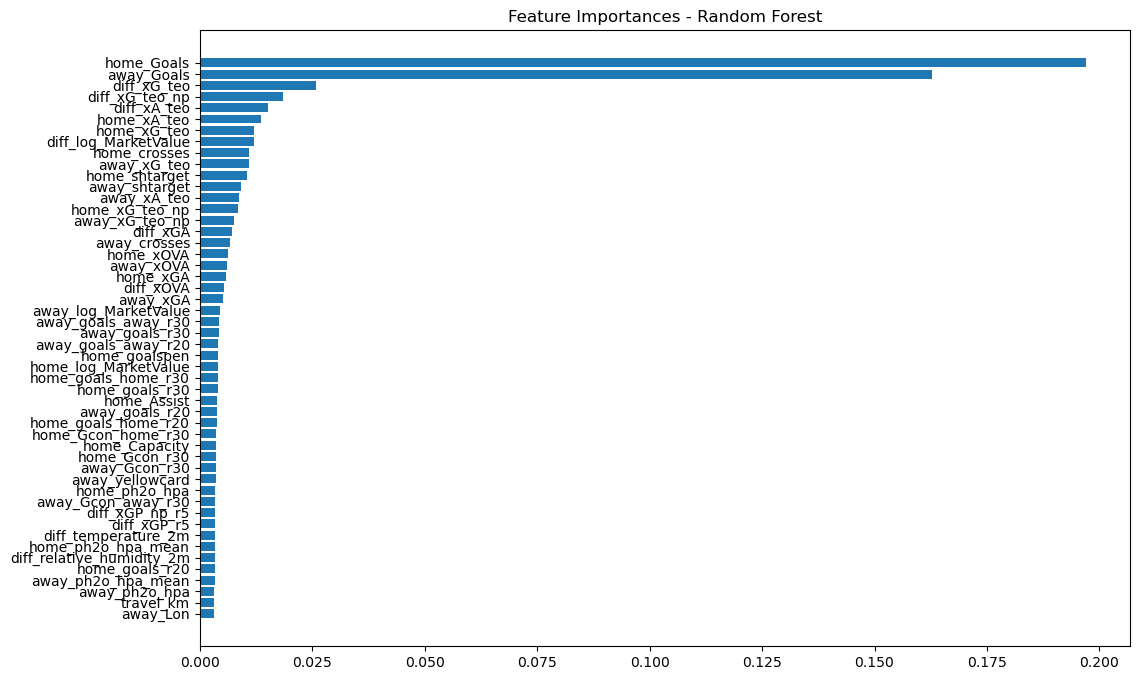
\includegraphics[width=\textwidth]{figures/primerforest.png}
		%\fbox{\parbox[c][4cm][c]{0.9\textwidth}{\centering \small [Figura: primerforest.png]}}
	\end{columns}
\end{frame}

% ---------- Slide 12: Segundo Random Forest ----------
\begin{frame}{Random Forest: segundo diagnóstico}{Señal genuina}
	\vspace*{-0.65cm}
	\begin{columns}[T,onlytextwidth]
		\column{.56\textwidth}
		\centering
		% PLACEHOLDER: figura de importancias del segundo RF
		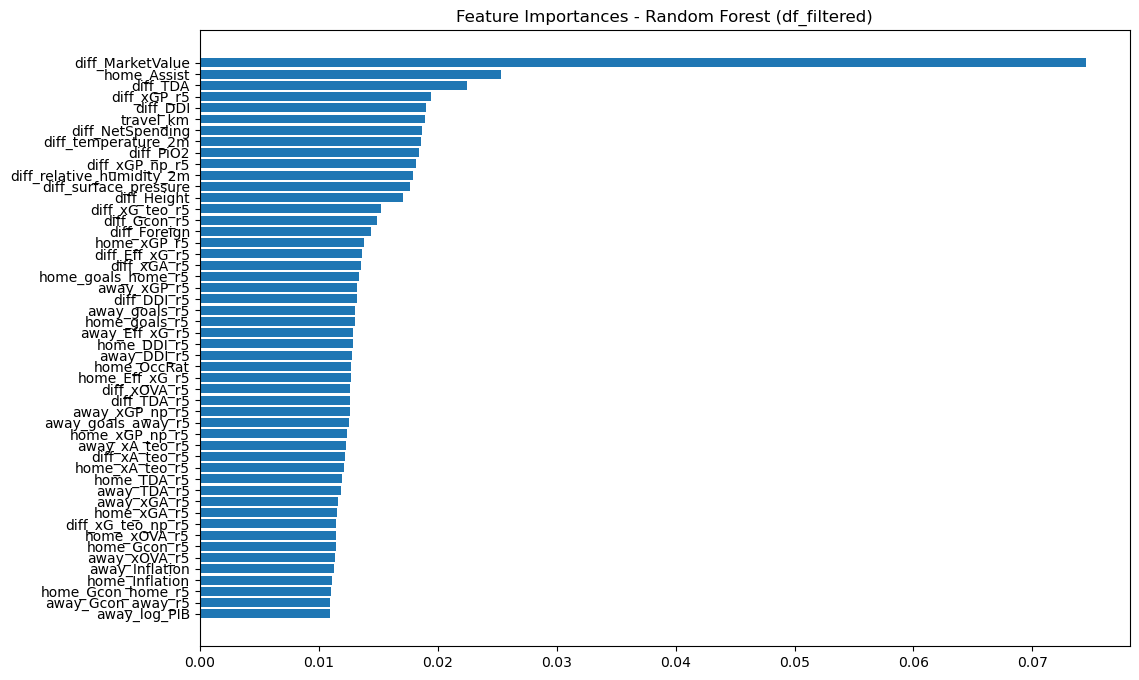
\includegraphics[width=\textwidth]{figures/segundoforest.png}
		%\fbox{\parbox[c][3.5cm][c]{0.9\textwidth}{\centering \small [Figura: segundoforest.png]}}
		\column{.40\textwidth}
		\footnotesize
		\begin{itemize}
			\item Accuracy cae a $0{.}4879$.
			\item Las importancias se reparten: \texttt{diff\_MarketValue} ($0{.}0745$), \texttt{home\_Assist} ($0{.}0253$), \texttt{diff\_TDA} ($0{.}0224$), \texttt{diff\_xGP\_r5} ($0{.}0194$).
			\item La clase empate colapsa: \emph{recall} de $0{.}03$.
			\item Predecir fútbol es un problema de alta entropía cuando se restringe a información previa al partido.
		\end{itemize}
	\end{columns}
\end{frame}

% ---------- Slide 14: Comparativa de los dos RF ----------
\begin{frame}{Random Forest: comparativa}{Los dos diagnósticos frente a frente}
	\begin{columns}[T,onlytextwidth]
		\column{.44\textwidth}
		\small
		\begin{itemize}
			\item Accuracy: $0{.}9078 \to 0{.}4879$.
			\item F1-weighted: $0{.}91 \to$ F1-macro $0{.}37$.
			\item La caída de 42 puntos confirma la fuga del primer modelo.
		\end{itemize}
		\column{.52\textwidth}
		\centering
		\scriptsize
		\renewcommand{\arraystretch}{1.2}
		\resizebox{0.95\textwidth}{!}{%
		\begin{tabular}{lccc|ccc}
			\toprule
			& \multicolumn{3}{c}{\textbf{Primer RF}} & \multicolumn{3}{c}{\textbf{Segundo RF}} \\
			\textbf{Clase} & Prec. & Rec. & F1 & Prec. & Rec. & F1 \\
			\midrule
			A & 0.93 & 0.93 & 0.93 & 0.48 & 0.38 & 0.43 \\
			D & 0.92 & 0.76 & 0.83 & 0.35 & 0.03 & 0.05 \\
			H & 0.89 & 0.98 & 0.93 & 0.49 & 0.84 & 0.62 \\
			\bottomrule
		\end{tabular}}%
	\end{columns}
\end{frame}

% ---------- Slide 15: Métricas deportivas ----------
\begin{frame}{M\'etricas deportivas}{\'Indices compuestos y promedios m\'oviles}
	\begin{columns}[T,onlytextwidth]
		\column{.50\textwidth}
		\tegetiqueta{\'Indices compuestos}\par\vskip 2mm
		\footnotesize
		\begin{itemize}
			\item $\text{xG\_teo} = 0{.}795 \cdot \text{attpen} + 0{.}358 \cdot \max(0, \text{shtarget} - \text{attpen})$
			\item $\text{xA\_teo} = 0{.}059 \cdot \text{crosses} + 0{.}0299 \cdot \text{foulsd}$
			\item $\text{DDI} = \dfrac{\text{TDA}}{\text{TDA} + \text{fouls} + \varepsilon} \text{.} \varepsilon>0 $
		\end{itemize}
		\column{.46\textwidth}
		\tegetiqueta{Promedios m\'oviles}\par\vskip 2mm
		\footnotesize
		\begin{itemize}
			\item Ventanas: 5, 10, 20 y 30 partidos.
			\item Goles: las cuatro ventanas.
			\item \'Indices compuestos: solo ventana de 5.
			\item Regla de inactividad: segmento se reinicia si el par\'on supera 40 días.
		\end{itemize}
	\end{columns}
	\vskip 1mm
	\secundario{\footnotesize Coeficientes calibrados sobre el panel y estudios t\'acticos externos.}
\end{frame}

% ---------- Slide 16: Covariables ambientales y geográficas ----------
\begin{frame}{Covariables ambientales y geogr\'aficas}{Dos asimetr\'ias f\'isicas distintas}
	\vspace*{-0.65cm}
	\begin{columns}[T,onlytextwidth]
		\column{.48\textwidth}
		\tegetiqueta{Distancia de viaje}\par\vskip 2mm
		\footnotesize F\'ormula de Haversine:
		\[
		\text{travel\_km} = 2R \arcsin(\sqrt{a})
		\]
		con
		\[
		a = \sin^2\!\left(\frac{\Delta\varphi}{2}\right) + \cos\varphi_1 \cos\varphi_2 \sin^2\!\left(\frac{\Delta\lambda}{2}\right)
		\]
		\secundario{\scriptsize $R = 6371$ km. $\varphi_i$: latitud. $\lambda_i$: longitud.}
		\column{.48\textwidth}
		\tegetiqueta{Presi\'on parcial de ox\'igeno}\par\vskip 2mm
		\footnotesize F\'ormula de Magnus:
		\[
		P_{\mathrm{H_2O}} = 6{.}112 \cdot e^{\frac{17{.}67\,T}{T + 243{.}5}} \cdot \frac{\mathrm{RH}}{100}
		\]
		\footnotesize Presi\'on parcial de ox\'igeno\supercite{West1996}:
		\[
		\mathrm{PiO_2} = (P_{\text{sup}} - P_{\mathrm{H_2O}}) \cdot 0{.}2095
		\]
	\end{columns}
\end{frame}

% ---------- Slide 17: Covariables econ\'omicas ----------
\begin{frame}{Covariables econ\'omicas}{}
	\footnotesize
	\begin{itemize}
		\item \texttt{diff\_MarketValue}: valor total de mercado del plantel.
		\item \texttt{diff\_NetSpending}: balance neto de transferencias.
		\item \texttt{diff\_Foreign}: número de jugadores extranjeros.
		\item \texttt{home\_Assist}: asistencia promedio al estadio del equipo local.
	\end{itemize}
	\footnotesize \textbf{Variables Descartadas:} \texttt{home\_OccRat} (vs \texttt{home\_Assist}, $\rho = 0{.}78$); PIB, inflaci\'on, IDE, Gini (baja señal predictiva, importancia $< 0{.}004$).
\end{frame}

% ---------- Slide 18: Datasets finales ----------
\begin{frame}{Datasets finales}{Tres conjuntos, dos exportados}
	\begin{columns}[T,onlytextwidth]
		\column{.48\textwidth}
		\centering
		\small
		\renewcommand{\arraystretch}{1.4}
		\resizebox{0.95\textwidth}{!}{%
		\begin{tabular}{l c c c}
			\toprule
			\textbf{Dataset} & \textbf{Partidos} & \textbf{Variables} & \textbf{Período} \\
			\midrule
			Lite & 37\,819 & 53 & 2017--2025 \\
			Full & 27\,067 & 56 & 2019--2025 \\
			Lite Recortado & 27\,067 & 53 & 2019--2025 \\
			\bottomrule
		\end{tabular}}%
		\column{.48\textwidth}
		\begin{minipage}{0.85\textwidth}
			\footnotesize
			\begin{itemize}
				\item \textbf{Lite:} ventana completa, sin \'indices compuestos de autor\'ia.
				\item \textbf{Full:} a\~nade \texttt{xG\_teo}, \texttt{xA\_teo}, \texttt{DDI} en ventana de 5.
				\item \textbf{Lite Recortado:} mismo per\'iodo que Full, sin \'indices. Permite comparaci\'on controlada.
			\end{itemize}
		\end{minipage}
	\end{columns}
\end{frame}

% =====================================================================
\section{Motor predictor G2Av1513}
% =====================================================================

% ---------- Slide 19: Bloque de conteo ----------
\begin{frame}{Bloque de conteo}{LightGBM Poisson $\to$ Skellam $\to$ $P_D^{(S)}$}
	\vspace*{-0.6cm}
	\begin{columns}[T,onlytextwidth]
		\column{.48\textwidth}
		\tegetiqueta{Modelo}\par\vskip 1mm
		\footnotesize
		\begin{itemize}
			\item Dos regresores LightGBM con funci\'on objetivo Poisson\supercite{ke2017lightgbm}.
			\item Predicen $\hat{\lambda}_H$ y $\hat{\lambda}_A$ a partir de 32 variables de rollings de goles.
			\item Hiperpar\'ametros: \texttt{n\_estimators}$=200$, \texttt{lr}$=0{.}05$, \texttt{depth}$=5$.
		\end{itemize}
		\column{.48\textwidth}
		\tegetiqueta{Probabilidad de empate}\par\vskip 1mm
		\footnotesize
		Distribuci\'on de Skellam\supercite{skellam1946,karlis2003} evaluada en $k=0$:
		\[
		\hat{P}_D^{(S)} = e^{-(\hat{\lambda}_H + \hat{\lambda}_A)} I_0\!\left(2\sqrt{\hat{\lambda}_H \hat{\lambda}_A}\right) 
		\]
		\secundario{\scriptsize $I_0$: funci\'on de Bessel modificada de orden cero.}
	\end{columns}
	\vskip 0.3mm
	\secundario{\footnotesize MAE $\in [0{.}836, 0{.}934]$ \quad$\cdot$\quad Calibraci\'on marginal del empate: sesgo $< 1$ pp.}
\end{frame}

% ---------- Slide 20: Modelo base (parte 1: estado y actualizaci\'on) ----------
\begin{frame}{Modelo base (1/2)}{Estado y actualizaci\'on secuencial}
	\vspace*{-0.7cm}
	\small
	\begin{itemize}
		\item \textbf{Rating efectivo del local:} $\tilde{\mu} = \mu + h$
		{\footnotesize Incorpora la ventaja de local\'ia sin alterar el rating base.}
		\vskip 0.5mm
		
		\item \textbf{Funci\'on de atenuaci\'on:} $g(\phi_j) = \frac{1}{\sqrt{1 + \dfrac{3\phi_j^2}{\pi^2}}}$
		{\footnotesize Pondera la incertidumbre del oponente.\supercite{Glickman2022}}
		\vskip 0.5mm
		
		\item \textbf{Operador de actualizaci\'on:} $\mu' = \mu + \phi'^2 \, g(\phi_j)\bigl(s_j - P_H\bigr)$
		{\footnotesize Corrige seg\'un el error de predicci\'on.}
	\end{itemize}
\end{frame}

% ---------- Slide 21: Modelo base (parte 2: probabilidades del resultado) ----------
\begin{frame}{Modelo base (2/2)}{Probabilidades del resultado}
	\footnotesize
	Se definen dos t\'erminos auxiliares:
	\[
	A = \exp\bigl(g(\phi_j)(\tilde{\mu} - \mu_j)\bigr), \qquad
	B = \exp(d + s)
	\]
	\vskip 1mm
	Las tres probabilidades del resultado son:
	\begin{equation*}
		P_H = \frac{A}{1 + A + B} \text{ , }
		P_D = \frac{B}{1 + A + B} \text{ , }
		P_A = \frac{1}{1 + A + B}
	\end{equation*}\supercite{Glicko2Mod}
	\vskip 1mm
	\secundario{\footnotesize $s$ es la probabilidad de empate derivada de la distribuci\'on de Skellam.}
\end{frame}

% ---------- Slide 22: Las 3 correcciones del G2Av1513 ----------
\begin{frame}{Modelo G2Av1513}{Correcciones y ajustes al Glicko-2 modificado\supercite{Glicko2Mod}}
	\centering
	\scriptsize
	\renewcommand{\arraystretch}{1.4}
	\resizebox{0.92\textwidth}{!}{%
		\begin{tabular}{p{3.2cm} p{5.2cm} p{5.2cm}}
			\toprule
			\textbf{Cambio} & \textbf{Original (Shelopugin-Sirotkin)} & \textbf{G2Av1513} \\
			\midrule
			Denominador trinomial &
			Asim\'etrico: dos denominadores distintos. Empate penalizado. &
			Sim\'etrico: $1 + e^{\delta} + e^{d + P_{D,\text{logit}}^{(S)}}$. Partici\'on consistente del simplex. \\
			Reparametrizaci\'on del empate &
			$P_D^{(S)} \in (0,1)$. &
			$P_{D,\text{logit}}^{(S)} = (P_D^{(S)}/1-P_D^{(S)})$. \\
			Constante de atenuaci\'on $g$ &
			$1{.}5/\pi^2$. &
			$3{.}0/\pi^2$.\\
			Volatilidad $\tau$ &
			$1{.}0$ &
			$0{.}8$ \\
			Desviaci\'on inicial $RD_0$ &
			$350$. &
			$80$. \\
			\bottomrule
	\end{tabular}}%
\end{frame}

% ---------- Slide 23: Evaluaci\'on aislada del G2Av1513 ----------
\begin{frame}{Evaluaci\'on aislada del motor}{L\'inea base antes del refinamiento}
	\begin{columns}[T,onlytextwidth]
		\column{.52\textwidth}
		\centering
		\small
		\renewcommand{\arraystretch}{1.4}
		\resizebox{\textwidth}{!}{%
			\begin{tabular}{lccc}
				\toprule
				\textbf{Dataset} & \textbf{LL Cat.} & \textbf{LL Bin.} & \textbf{LL OVR} \\
				\midrule
				Full & 1.0425 & 0.6496 & 0.6064 \\
				Lite & 1.0412 & 0.6473 & 0.6058 \\
				Lite Rec. & 1.0425 & 0.6496 & 0.6064 \\
				\bottomrule
		\end{tabular}}%
		\column{.44\textwidth}
		\tegetiqueta{Lectura}\par\vskip 2mm
		\small
		\begin{itemize}
			\item Cota sin informaci\'on: $\ln 3 \approx 1{.}099$.
			\item El motor se ubica por debajo: hay se\~nal predictiva genuina.
			\item Esta tabla es la l\'inea base contra la cual se mide el MLP.
		\end{itemize}
	\end{columns}
\end{frame}

% ---------- Slide 24: Ventaja de local\'ia por liga ----------
\begin{frame}{Ventaja de local\'ia por liga}{Top 5 y bottom 5}
	\vspace*{-0.75cm}
	\begin{columns}[T,onlytextwidth]
		\column{.45\textwidth}
		\tegetiqueta{Top 5}\par\vskip 2mm
		\centering
		\footnotesize
		\renewcommand{\arraystretch}{1.3}
		\resizebox{0.92\textwidth}{!}{%
		\begin{tabular}{lcc}
			\toprule
			\textbf{Competici\'on} & \textbf{Lite} & \textbf{Full} \\
			\midrule
			Major League Soccer & 60.46 & 51.90 \\
			Brasileir\~ao & 54.44 & 51.58 \\
			CONCACAF Champions League & 52.42 & 52.04 \\
			FIFA Club World Cup & 50.51 & 50.19 \\
			AFC Champions League Elite & 50.08 & --- \\
			\bottomrule
		\end{tabular}}%
		\column{.45\textwidth}
		\tegetiqueta{Bottom 5}\par\vskip 2mm
		\centering
		\footnotesize
		\renewcommand{\arraystretch}{1.3}
		\resizebox{0.8\textwidth}{!}{%
		\begin{tabular}{lcc}
			\toprule
			\textbf{Competici\'on} & \textbf{Lite} & \textbf{Full} \\
			\midrule
			J1 League & 19.04 & 14.55 \\
			Persian Gulf Pro League & 19.68 & --- \\
			Ligue 1 & 21.59 & 21.10 \\
			K League 1 & 22.29 & 18.45 \\
			Premier League & 26.31 & 25.72 \\
			\bottomrule
		\end{tabular}}%
	\end{columns}
	\vskip 1mm
	\secundario{\footnotesize Los ratings iniciales por liga permanecen pr\'oximos a 1500 ($|\mu_\text{init} - 1500| < 0{.}06$).}
\end{frame}

% =====================================================================
\section{Refinamiento neuronal}
% =====================================================================

% ---------- Slide 25: Arquitectura del MLP ----------
\begin{frame}{Refinamiento neuronal}{Arquitectura del perceptr\'on multicapa}
	\centering
	\vspace*{-0.2cm}
	\resizebox{0.98\textwidth}{!}{%
		\begin{tikzpicture}[
			capa/.style={rectangle, draw=tegAcento, fill=tegGrisClaro,
				rounded corners, text width=2.6cm, align=center,
				minimum height=1.4cm, font=\small},
			arrow/.style={-{Stealth[length=3mm]}, thick, tegAcento},
			node distance=0.6cm and 0.7cm
			]
			\node[capa] (in) {Entrada\\$3 + p$};
			\node[capa, right=of in] (h1) {64 neuronas\\ReLU\supercite{Charu2018} + Dropout $0{.}3$};
			\node[capa, right=of h1] (h2) {64 neuronas\\ReLU\supercite{Charu2018} + Dropout $0{.}3$};
			\node[capa, right=of h2] (out) {Salida\\3 neuronas\\softmax};
			
			\draw[arrow] (in) -- (h1);
			\draw[arrow] (h1) -- (h2);
			\draw[arrow] (h2) -- (out);
	\end{tikzpicture}}%
	\vskip 0.5mm
	\begin{columns}[T,onlytextwidth]
		\column{.48\textwidth}
		\tegetiqueta{Entrada}\par\vskip 2mm
		\footnotesize
		$(P_H, P_D, P_A)$ + covariables ex\'ogenas estandarizadas.
		\begin{itemize}
			\item $p = 7$ en Lite y Lite Recortado.
			\item $p = 10$ en Full.
		\end{itemize}
		\column{.48\textwidth}
		\tegetiqueta{Entrenamiento}\par\vskip 2mm
		\footnotesize
		\begin{itemize}
			\item P\'erdida: entrop\'ia cruzada categ\'orica.
			\item Optimizador: Adam, $\eta_0 = 10^{-3}$\supercite{loshchilov2017adamw}.
			\item $50$ \'epocas, lotes de $64$.
		\end{itemize}
	\end{columns}
\end{frame}

% ---------- Slide 26: Protocolo experimental ----------
\begin{frame}{Protocolo experimental}{Diez ejecuciones pareadas}
	\vspace*{-0.7cm}
	\begin{columns}[T,onlytextwidth]
		\column{.48\textwidth}
		\tegetiqueta{Dise\~no}\par\vskip 2mm
		\footnotesize
		\begin{itemize}
			\item \textbf{10 ejecuciones}, \texttt{SEED=42-51}.
			\item El Glicko-2 se recalibra en cada ejecuci\'on con par\'ametros fijos.
			\item Configuraciones del MLP: Base y Completo
		\end{itemize}
		\column{.48\textwidth}
		\tegetiqueta{Contraste}\par\vskip 2mm
		\footnotesize
		Test $t$ pareado \supercite{hernandezBenito} sobre las diferencias por ejecuci\'on:
		\[
		\Delta_k = \mathcal{M}_k^{\text{base}} - \mathcal{M}_k^{\text{completo}}
		\]
		\[
		t = \frac{\bar{\Delta}}{s_\Delta / \sqrt{K}}, \quad K = 10
		\]
		\secundario{\scriptsize $p$-valor bajo $t$ de Student con $K-1$ grados de libertad.}
	\end{columns}
	\vskip 1mm
	\secundario{\scriptsize Se ejecutan 6 redes en total: 2 configuraciones $\times$ 3 datasets.}
\end{frame}

% ---------- Slide 27: Resultados del MLP ----------
\begin{frame}{Resultados del refinamiento}{M\'etricas probabil\'isticas}
	\vspace*{-0.6cm}
	\centering
	\scriptsize
	\renewcommand{\arraystretch}{1.3}
	\resizebox{0.85\textwidth}{!}{%
		\begin{tabular}{l l c c c c}
			\toprule
			\textbf{Dataset} & \textbf{Config.} & \textbf{LL Cat.} & \textbf{LL Bin.} & \textbf{Acc.} & \textbf{$F1_D$} \\
			\midrule
			Full & Base & $1.0248 \pm 0.0002$ & $0.6443 \pm 0.0002$ & $0.485$ & $0.0000$ \\
			& Completo & $1.0261 \pm 0.0004$ & $0.6440 \pm 0.0003$ & $0.489$ & $0.0043 \pm 0.0025$ \\
			\midrule
			Lite & Base & $1.0227 \pm 0.0002$ & $0.6410 \pm 0.0001$ & $0.487$ & $0.0000$ \\
			& Completo & $1.0226 \pm 0.0006$ & $0.6402 \pm 0.0005$ & $0.489$ & $0.0075 \pm 0.0014$ \\
			\midrule
			Lite Rec. & Base & $1.0247 \pm 0.0002$ & $0.6449 \pm 0.0002$ & $0.485$ & $0.0000$ \\
			& Completo & $1.0276 \pm 0.0005$ & $0.6457 \pm 0.0005$ & $0.486$ & $0.0015 \pm 0.0006$ \\
			\bottomrule
	\end{tabular}}%
	\vskip 1mm
	\secundario{\footnotesize El refinamiento reduce la LL Cat. entre $0{.}0149$ y $0{.}0185$ respecto al Glicko-2 aislado.\supercite{gneiting2007}}
\end{frame}

% ---------- Slide 28: Trade-off (test t) ----------
\begin{frame}{El intercambio}{Mejora el empate, deteriora la calibraci\'on global}
	\vspace*{-0.15cm}
	\begin{columns}[T,onlytextwidth]
		\column{.4\textwidth}
		\centering
		\footnotesize
		\renewcommand{\arraystretch}{1.3}
		\resizebox{\textwidth}{!}{%
			\begin{tabular}{lccc}
				\toprule
				& \multicolumn{3}{c}{\textbf{Test $t$ pareado}} \\
				\textbf{Dataset} & \textbf{LL Cat.} & \textbf{LL Bin.} & \textbf{$F1_D$} \\
				\midrule
				Full & $-5.53^{*}$ & $1.88$ & $-3.42^{*}$ \\
				Lite & $1.04$ & $10.65^{*}$ & $-5.54^{*}$ \\
				Lite Rec. & $-15.25^{*}$ & $-9.95^{*}$ & $-3.08^{*}$ \\
				\bottomrule
		\end{tabular}}%
		\newline
		\secundario{\scriptsize $^{*}$: significativo al $5\%$. Signo positivo: mejora el modelo completo.}
		\column{.46\textwidth}
		\tegetiqueta{Lectura}\par\vskip 2mm
		\footnotesize
		\begin{itemize}
			\item De 4 efectos significativos, \textbf{3 deterioran} la calibraci\'on global.
			\item El $F1_D$ mejora significativamente en los 3 datasets.
			\item Magnitud: $\sim 10^{-3}$ en escala de log-loss.
		\end{itemize}
	\end{columns}
	\vskip 0.5mm
	\secundario{\footnotesize Las covariables empujan masa hacia el empate: mejora la clase $D$, distorsiona el simplex.}
\end{frame}

% ---------- Slide 29: Colapso del empate ----------
\begin{frame}{El colapso del empate}{No es un bug, es el simplex}
	\vspace*{-0.6cm}
	\begin{columns}[T,onlytextwidth]
		\column{.48\textwidth}
		\tegetiqueta{Configuraci\'on base}\par\vskip 2mm
		\footnotesize
		\begin{itemize}
			\item $F1_D \equiv 0$ en las 30 ejecuciones.
			\item $\arg\max$ nunca predice $D$.
			\item Masa desplazada a $H$ o $A$ por asimetr\'ia estructural.
		\end{itemize}
		\column{.48\textwidth}
		\tegetiqueta{Configuraci\'on completa}\par\vskip 2mm
		\footnotesize
		\begin{itemize}
			\item $F1_D > 0$ predice cercano a la frecuencia natural ($0{.}267$)
			\item \textbf{Precisi\'on:} Full: $0{.}206$, Lite: $0{.}270$, Lite Rec.: $0{.}214$.
			\item Covariables expanden la regi\'on de dominio de $D$.
		\end{itemize}
	\end{columns}
	\vskip 2mm
	\secundario{\footnotesize La log-loss penaliza la distorsi\'on del simplex. El $F1_D$ mide solo la frontera de decisi\'on.}
\end{frame}

% ---------- Slide 30: Cierre del bloque de resultados (cifras) ----------
\begin{frame}{Cierre del flujo en cascada}{Motor aislado y refinamiento | log-loss categ\'orica}
	\vspace*{-0.4cm}
	\centering
	\begin{columns}[T,onlytextwidth]
		\column{.32\textwidth}
		\centering
		\scalebox{0.6}{%
		\begin{minipage}{1.6\textwidth}
		\centering
		\tegetiqueta{Full}\par\vskip 3mm
		\cifra{1{.}0425}{Glicko-2 aislado}\par\vskip 2mm
		\cifra{1{.}0248}{MLP base}\par\vskip 2mm
		\cifra{1{.}0261}{MLP completo}
		\end{minipage}}%
		\column{.32\textwidth}
		\centering
		\scalebox{0.6}{%
		\begin{minipage}{1.6\textwidth}
		\centering
		\tegetiqueta{Lite Rec.}\par\vskip 3mm
		\cifra{1{.}0425}{Glicko-2 aislado}\par\vskip 2mm
		\cifra{1{.}0248}{MLP base}\par\vskip 2mm
		\cifra{1{.}0276}{MLP completo}
		\end{minipage}}%
		\column{.32\textwidth}
		\centering
		\scalebox{0.6}{%
		\begin{minipage}{1.6\textwidth}
		\centering
		\tegetiqueta{Lite}\par\vskip 3mm
		\cifra{1{.}0412}{Glicko-2 aislado}\par\vskip 2mm
		\cifra{1{.}0227}{MLP base}\par\vskip 2mm
		\cifra{1{.}0226}{MLP completo}
		\end{minipage}}%
		\end{columns}
		\vfill
		\secundario{\small El refinamiento reduce la log-loss categ\'orica.}
\end{frame}

% ---------- Slide 31: Destacado ----------
\destacado[Resultado central]{El sistema en cascada predice mejor que el azar con una muestra reducida y corrige parcialmente un problema estructural del modelo.}

% ---------- Slide 32: Bisagra hacia ap\'endices ----------
\begin{frame}{S\'intesis}{¿Base para nuevas exploraciones?}
	\vspace*{-6mm}
	\begin{columns}[T,onlytextwidth]
		\column{.48\textwidth}
		\tegetiqueta{Lo que se explor\'o}\par\vskip 2mm
		\footnotesize
		\begin{itemize}
			\item Modelo auxiliar de conteo: de goles a $P_{D}^{(S)}$.
			\item Inyecci\'on de una tercera categor\'ia en un sistema binario.
			\item Refinamiento mediante una red neuronal.
			\item Cuales de los torneos poseen una fuerte ventaja local.
		\end{itemize}
		\column{.48\textwidth}
		\tegetiqueta{¿Qu\'e m\'as se puede explorar a part\'ir de esto?}\par\vskip 2mm
		\footnotesize
		\begin{itemize}
			\item ¿Podr\'ia una red neuronal sustituir el sistema en cascada?
			\item ¿Qu\'e pasar\'ia si no se calibra el modelo?
			\item ¿Se puede proyectar la evoluci\'on futura de ratings?
		\end{itemize}
	\end{columns}
\end{frame}
% =====================================================================
\section{Estudios Exploratorios}
% =====================================================================

% ---------- Slide 30: GRU Motivacion y arquitectura ----------
\begin{frame}{Ap\'endice A: \textit{Gated Recurrent Unit}}{Motivaci\'on y Arquitectura}
	\begin{columns}[T,onlytextwidth]
		\column{.48\textwidth}
		\tegetiqueta{Motivaci\'on}\par\vskip 2mm
		\footnotesize
		\begin{itemize}
			\item Modelar expl\'icitamente la secuencia de partidos.
			\item Alternativa puramente secuencial al estado $(R, RD, \sigma)$ del Glicko-2.
		\end{itemize}
		\column{.48\textwidth}
		\tegetiqueta{Arquitectura}\par\vskip 2mm
		\footnotesize
		\begin{itemize}
			\item Pesos compartidos entre ambos codificadores.
			\item $h = 64$ neuronas ocultas.
		\end{itemize}
	\end{columns}
\end{frame}


% ---------- Slide 31: GRU Arquitectura ----------
\begin{frame}{Ap\'endice A: \textit{Gated Recurrent Unit}}{Arquitectura (Diagrama)}
	\centering
	\resizebox{0.85\textwidth}{!}{%
		\begin{tikzpicture}[
			caja/.style={rectangle, draw=tegAcento, fill=tegGrisClaro,
				rounded corners, text width=2.4cm, align=center,
				minimum height=1cm, font=\small},
			gru/.style={rectangle, draw=tegAcentoMedio, fill=tegGrisClaro,
				rounded corners, text width=2.6cm, align=center,
				minimum height=1.4cm, font=\small},
			arrow/.style={-{Stealth[length=3mm]}, thick, tegAcento},
			node distance=0.7cm and 0.9cm
			]
			\node[gru] (gh) {GRU local\\$T = 8$};
			\node[gru, below=0.8cm of gh] (ga) {GRU visitante\\$T = 8$};
			\node[caja, right=1.4cm of gh] (cat) {Concatenaci\'on};
			\node[caja, right=of cat] (head) {Densa\\ReLU + dropout};
			\node[caja, right=of head] (out) {Softmax\\3 salidas};
			
			\draw[arrow] (gh) -- (cat);
			\draw[arrow] (ga) -- (cat);
			\draw[arrow] (cat) -- (head);
			\draw[arrow] (head) -- (out);
	\end{tikzpicture}}%
\end{frame}

% ---------- Slide 32: GRU Resultados ----------
\begin{frame}{Ap\'endice A: \textit{Gated Recurrent Unit}}{Resultados emp\'iricos}
	\begin{columns}[T,onlytextwidth]
		\column{.46\textwidth}
		\centering
		\scriptsize
		\renewcommand{\arraystretch}{1.3}
		\resizebox{\textwidth}{!}{%
			\begin{tabular}{lccc}
				\toprule
				\textbf{Dataset} & \textbf{Modelo} & \textbf{LL Cat.} & \textbf{Acc.} \\
				\midrule
				Full & G2A aislado & 1.0425 & --- \\
				& MLP completo & 1.0261 & 0.489 \\
				& GRU & 1.1027 & 0.438 \\
				\midrule
				Lite & G2A aislado & 1.0412 & --- \\
				& MLP completo & 1.0226 & 0.489 \\
				& GRU & 1.0535 & 0.466 \\
				\bottomrule
		\end{tabular}}%
		\column{.50\textwidth}
		\tegetiqueta{Lectura}\par\vskip 2mm
		\footnotesize
		\begin{itemize}
			\item La GRU rinde por debajo del G2A aislado.
			\item Sobreajuste estructural.
			\item Informaci\'on temporal ya condensada en promedios m\'oviles y el estado $(R, RD, \sigma)$.
		\end{itemize}
	\end{columns}
\end{frame}

% ---------- Slide 32: NAIVE Qu\'e es el motor naive ----------
\begin{frame}{Ap\'endice B: Naive vs G2Av1513}{Modelo Naive: Glicko-2 Shelopugin-Sirotkin, sin calibrar}
	\vspace*{-0.6cm}
	\begin{columns}[T,onlytextwidth]
		\column{.48\textwidth}
		\tegetiqueta{Par\'ametros fijos}\par\vskip 2mm
		\footnotesize
		\begin{itemize}
			\item $RD_0 = 350$.
			\item $\tau = 1{.}0$.
			\item $g_{\text{const}} = 1{.}5/\pi^2$.
			\item $d = 0$ (sin correcci\'on de empate).
			\item $h = 0$ (sin ventaja de local\'ia).
			\item $R_0 = 1500$ universal.
		\end{itemize}
		\column{.48\textwidth}
		\tegetiqueta{Dise\~no}\par\vskip 2mm
		\footnotesize
		\begin{itemize}
			\item Sin optimizaci\'on de hiperpar\'ametros.
			\item No distingue ligas ni contextos temporales.
			\item Inyecta $P_D^{(S)}$ crudo, sin transformaci\'on logit.
			\item Punto de partida: cuantificar el aporte de la calibraci\'on.
		\end{itemize}
	\end{columns}
	\vskip 2mm
	\secundario{\footnotesize El motor naive no es el Shelopugin-Sirotkin: incorpora sus mejoras, pero sin calibraci\'on.}
\end{frame}

% ---------- Slide 34: NAIVE Comparativa de hiperpar\'ametros ----------
\begin{frame}{Ap\'endice B: Naive vs G2Av1513}{Comparativa de hiperpar\'ametros}
	\vspace*{-0.2cm}
	\centering
	\scriptsize
	\renewcommand{\arraystretch}{1.3}
	\resizebox{0.9\textwidth}{!}{%
		\begin{tabular}{p{3.2cm} p{4.2cm} p{5.0cm}}
			\toprule
			\textbf{Componente} & \textbf{Motor naive} & \textbf{Motor G2Av1513} \\
			\midrule
			$RD_0$ & $350$ & $80$ \\
			$g_{\text{const}}$ & $1{.}5/\pi^2$ & $3{.}0/\pi^2$ \\
			Denominador trinomial & Asim\'etrico & Sim\'etrico \\
			Transformaci\'on de $P_D$ & Crudo $(0,1)$ & $\operatorname{logit}(P_D^{(S)})$ \\
			Par\'ametro $d$ & Fijo ($0$) & Calibrado ($\approx 0{.}91$) \\
			Calibraci\'on param\'etrica & Ninguna & L-BFGS-B \\
			Ventaja de local\'ia & Fija ($0$) & Calibrada por liga \\
			Rating inicial & $1500$ universal & $\mu_{\text{init},\ell}$ por liga \\
			Estabilidad num\'erica & M\'inima & Clamping, restricci\'on, etc. \\
			\bottomrule
	\end{tabular}}%
	\vskip 1mm
	\secundario{\footnotesize La calibraci\'on estructural es el verdadero habilitador del poder predictivo.\supercite{Glickman2022}}
\end{frame}

% ---------- Slide 35: NAIVE Concordancia y discrepancias ----------
\begin{frame}{Ap\'endice B: Naive vs G2Av1513}{Concordancia y casos extremos}
	\begin{columns}[T,onlytextwidth]
		\column{.46\textwidth}
		\centering
		\scriptsize
		\renewcommand{\arraystretch}{1.3}
		\resizebox{\textwidth}{!}{%
			\begin{tabular}{lccc}
				\toprule
				\textbf{Dataset} & \textbf{Spearman} & $\overline{|\Delta\mu|}$ & $\overline{|\Delta \text{Rank}|}$ \\
				\midrule
				Full & $0.9416$ & $40.67$ & $23.31$ \\
				Lite & $0.9260$ & $51.31$ & $33.23$ \\
				Lite Rec. & $0.9416$ & $40.67$ & $23.31$ \\
				\bottomrule
		\end{tabular}}%
		\vskip 3mm
		\secundario{\scriptsize $\rho > 0{.}92$: la jerarqu\'ia competitiva se preserva.\supercite{spearman1904}}
		\column{.50\textwidth}
		\tegetiqueta{Discrepancias extremas (Lite)}\par\vskip 2mm
		\footnotesize
		\begin{itemize}
			\item CSA (Brasileir\~ao): $|\Delta\mu| = 183{.}13$.
			\item Platanias (Grecia): $|\Delta\mu| = 166{.}05$.
			\item Southampton (PL): $|\Delta\mu| = 142{.}42$.
		\end{itemize}
		\vskip 2mm
		\secundario{\scriptsize La \'elite global (PSG, Bayern, Real Madrid) permanece pr\'acticamente inalterada ($|\Delta\mu| < 53$).}
	\end{columns}
\end{frame}

% ---------- Slide 36: LSTMvARIMA Panel semanal ----------
\begin{frame}{Ap\'endice C: Proyecci\'on ARIMA y LSTM}{Panel semanal}
	\begin{columns}[T,onlytextwidth]
		\column{.48\textwidth}
		\tegetiqueta{Unidad temporal}\par\vskip 2mm
		\footnotesize
		\begin{itemize}
			\item Semana (\texttt{W-MON}, ancla en lunes).
			\item Calendarios asincr\'onicos: ligas europeas (interanual) vs americanas/asi\'aticas (anual).
			\item Una unidad diaria dar\'ia $>90\%$ de faltantes.
		\end{itemize}
		\column{.48\textwidth}
		\tegetiqueta{Construcci\'on}\par\vskip 2mm
		\footnotesize
		\begin{itemize}
			\item \texttt{ffill} con l\'imite de 30 semanas (par\'on vacacional europeo).
			\item Full: 334 equipos, 346 semanas.
			\item Lite: 412 equipos, 424 semanas.
			\item Split cronol\'ogico: 70/30.
		\end{itemize}
	\end{columns}
	\vfill
	\secundario{\footnotesize La semana es la unidad m\'inima que garantiza al menos una observaci\'on por equipo.}
\end{frame}

% ---------- Slide 36: LSTMvARIMA LSTM y ARIMA ----------
\begin{frame}{Ap\'endice C: Proyecci\'on ARIMA y LSTM}{ARIMA y LSTM}
	\vspace*{-0.6cm}
	\begin{columns}[T,onlytextwidth]
		\column{.48\textwidth}
		\tegetiqueta{ARIMA}\par\vskip 2mm
		\footnotesize
		\begin{itemize}
			\item Modelo univariado por equipo.
			\item Cap: \texttt{max\_p}$=3$, \texttt{max\_q}$=3$, \texttt{max\_d}$=2$.
			\item Timeout de 60 s por equipo.
			\item Predicci\'on \textit{one-step ahead} con actualizaci\'on secuencial.
		\end{itemize}
		\column{.48\textwidth}
		\tegetiqueta{LSTM global}\par\vskip 2mm
		\footnotesize
		\begin{itemize}
			\item Red \'unica entrenada sobre todos los equipos.
			\item Secuencias de $T = 8$ semanas, 64 unidades.
			\item Escalado \texttt{StandardScaler} por equipo (ajustado solo en train).
			\item Early stopping con paciencia 5.
		\end{itemize}
	\end{columns}
	\vskip 1mm
	\secundario{\footnotesize ARIMA: precisi\'on univariada. LSTM: patrones compartidos entre equipos.}
\end{frame}


% ---------- Slide 37: LSTMvARIMA M\'etricas globales ----------
\begin{frame}{Ap\'endice C: Proyecci\'on ARIMA y LSTM}{M\'etricas globales}
	\vspace*{-0.6cm}
	\begin{columns}[T,onlytextwidth]
		\column{.50\textwidth}
		\centering
		\small
		\renewcommand{\arraystretch}{1.4}
		\resizebox{\textwidth}{!}{%
			\begin{tabular}{l c c c c}
				\toprule
				\textbf{Dataset} & \textbf{Modelo} & \textbf{RMSE} & \textbf{MAE} & \textbf{Spearman} \\
				\midrule
				Full & ARIMA & 6.8819 & 4.4250 & $0.9975$ \\
				& LSTM & 9.9615 & 7.1723 & $0.9966$ \\
				\midrule
				Lite & ARIMA & 10.0592 & 4.8542 & $0.9967$ \\
				& LSTM & 11.3669 & 6.3074 & $0.9964$ \\
				\bottomrule
		\end{tabular}}%
		\column{.46\textwidth}
		\tegetiqueta{Lectura}\par\vskip 2mm
		\footnotesize
		\begin{itemize}
			\item ARIMA gana en RMSE y MAE en ambos datasets.
			\item Ambos preservan el ranking ($\rho > 0{.}99$).
			\item LSTM solo supera a ARIMA en el $19{.}2\%$ (Full) y $33{.}6\%$ (Lite) de los equipos.
			\item LSTM \'util en series de alta volatilidad.
		\end{itemize}
	\end{columns}
\end{frame}

% ---------- Slide 38: LSTMvARIMA Series ARIMA vs LSTM ----------
\begin{frame}{Ap\'endice C: Proyecci\'on ARIMA y LSTM de ratings}{ARIMA vs LSTM}
	\vspace*{-0.6cm}
	\begin{columns}[T,onlytextwidth]
		\column{.50\textwidth}
		\centering
		\small
		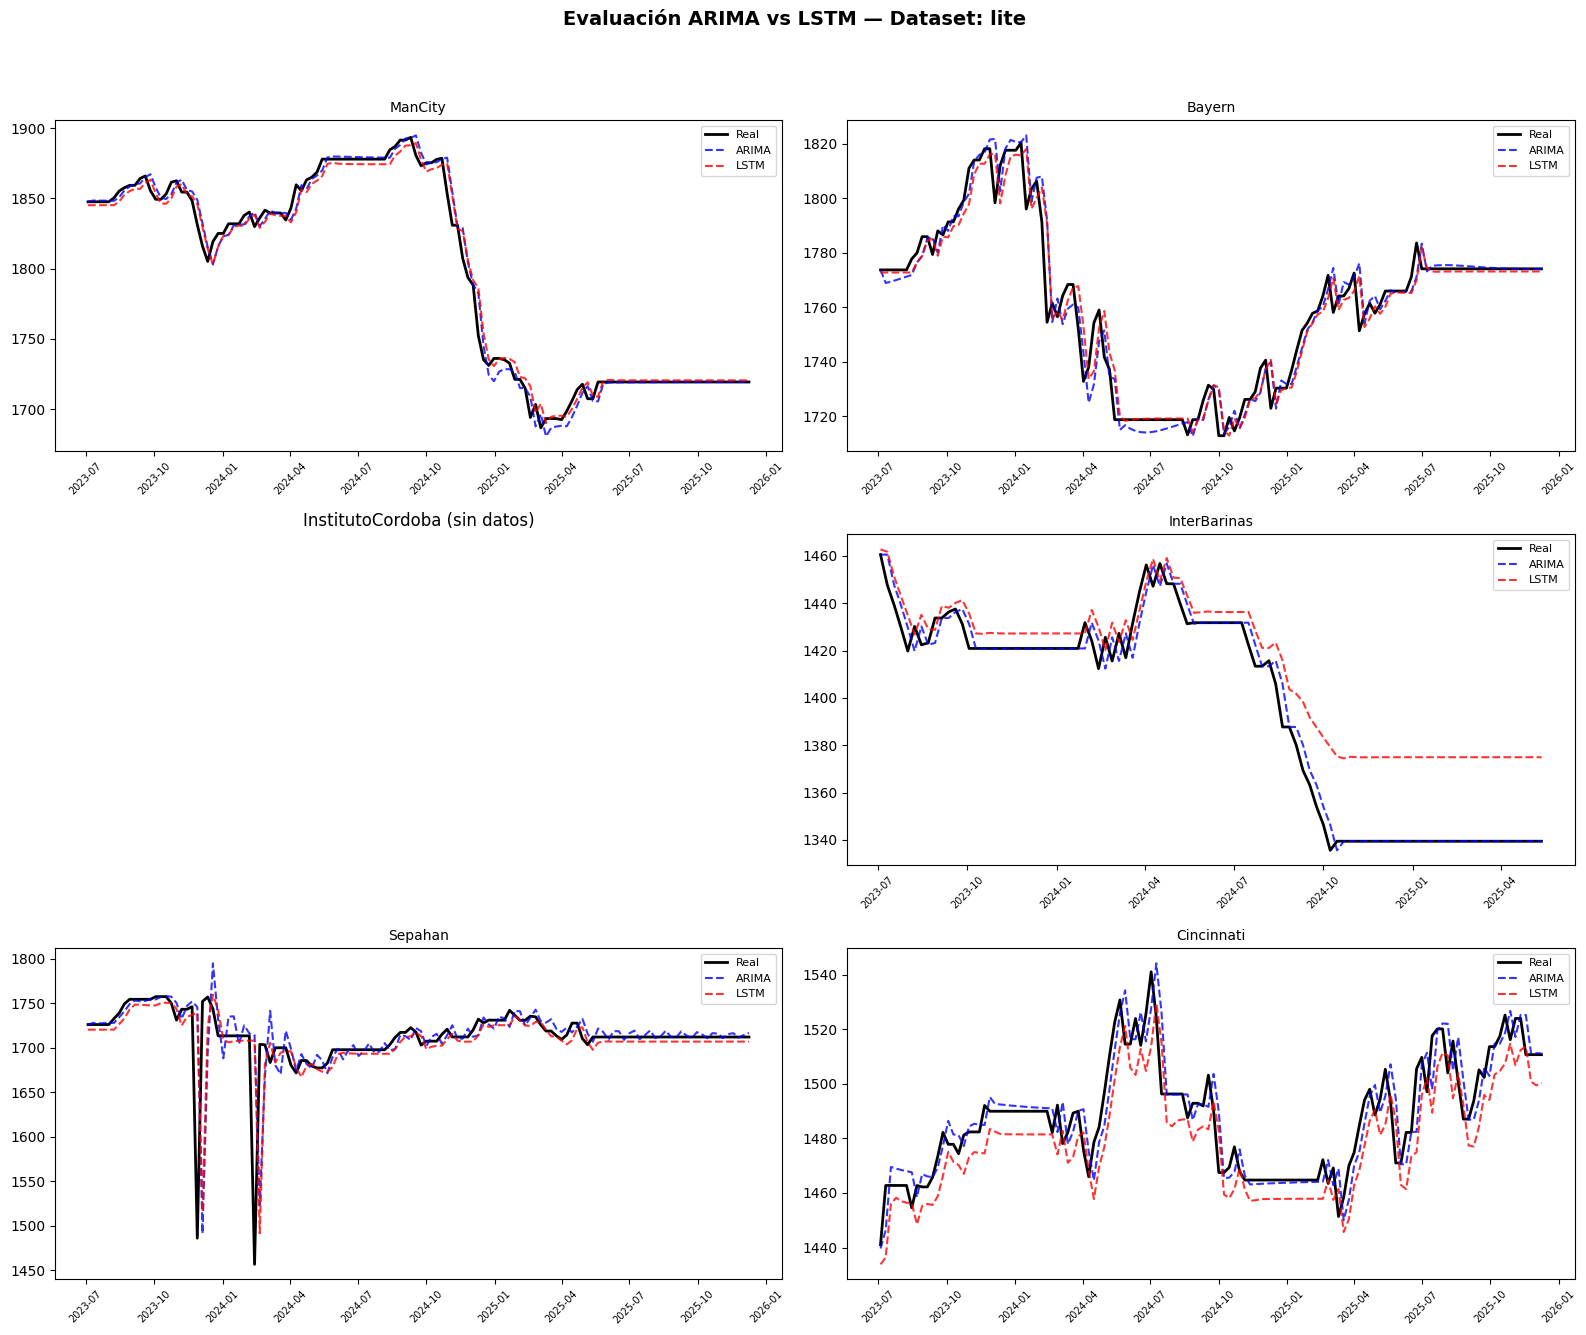
\includegraphics[width=0.6\textwidth]{figures/ARIMAvsLSTMlite.png}
		\column{.50\textwidth}
		\centering
		\small
		\begin{minipage}{0.9\textwidth}
		\footnotesize
		\begin{itemize}
			\item ARIMA oscila en parones prolongados y ca\'idas bruscas de $\mu$.
			\item LSTM amortigua esos rebotes, pero diverge en equipos con alta volatilidad.
			\item Elecci\'on: ARIMA para precisi\'on, LSTM para suavizado en series irregulares.
		\end{itemize}
		\end{minipage}
	\end{columns}
\end{frame}

% ---------- Slide 39: MODELOS M\'etricas de concordancia ----------
\begin{frame}{Ap\'endice D: Validaci\'on y nivel de poder}{Cuatro m\'etricas de concordancia}
	\vspace*{-0.6cm}
	\begin{columns}[T,onlytextwidth]
		\column{.48\textwidth}
		\tegetiqueta{Spearman $\rho$}\par\vskip 1mm
		\footnotesize
		Correlaci\'on de rangos\supercite{spearman1904}:
		\[
		\rho = \frac{\operatorname{cov}(R_1, R_2)}{\sigma_{R_1}\,\sigma_{R_2}}
		\]
		\vskip 2mm
		\tegetiqueta{Kendall $\tau$}\par\vskip 1mm
		\footnotesize
		Pares concordantes vs discordantes\supercite{kendall1945}:
		\[
		\tau = \frac{n_c - n_d}{\tfrac{1}{2}n(n-1)}
		\]
		\column{.48\textwidth}
		\tegetiqueta{Overlap@$K$}\par\vskip 1mm
		\footnotesize
		Proporci\'on de equipos en com\'un en el Top $K$:
		\[
		\text{Overlap}_K = \frac{|\mathcal{T}_K^{(1)} \cap \mathcal{T}_K^{(2)}|}{K}
		\]
		\vskip 2mm
		\tegetiqueta{MAE de posici\'on}\par\vskip 1mm
		\footnotesize
		Error posicional medio:
		\[
		\text{MAE} = \frac{1}{n}\sum_{i=1}^{n} |\text{rank}_i^{(1)} - \text{rank}_i^{(2)}|
		\]
	\end{columns}
\end{frame}

% ---------- Slide 40: MODELOS Tabla de validaciones ----------
\begin{frame}{Ap\'endice D: Validaci\'on y nivel de poder}{Validaci\'on vs Rankings institucionales\supercite{clubelo2025,kassiesa2025,conmebol2026,footyrankings2025}}
	\centering
	\scriptsize
	\renewcommand{\arraystretch}{1.3}
	\resizebox{0.8\textwidth}{!}{%
		\begin{tabular}{l c c c c c c}
			\toprule
			\textbf{Validaci\'on} & \textbf{N} & \textbf{Spearman} & \textbf{Kendall} & \textbf{Overlap@10} & \textbf{Overlap@20} & \textbf{MAE} \\
			\midrule
			UEFA 2025 & 44 & 0.655 & 0.479 & 0.700 & 0.750 & 8.1 \\
			ELO Ago 2025 & 79 & 0.787 & 0.612 & 0.700 & 0.700 & 11.4 \\
			AFC 2025 & 16 & 0.079 & 0.050 & 0.600 & 0.800 & 5.1 \\
			CONMEBOL 2026 & 77 & 0.645 & 0.471 & 0.600 & 0.600 & 13.9 \\
			LSTM vs UEFA 2026 & 47 & 0.708 & 0.543 & 0.900 & 0.700 & 7.4 \\
			LSTM vs ELO Sep 2026 & 273 & 0.472 & 0.332 & 0.600 & 0.650 & 61.4 \\
			LSTM vs AFC 2026 & 15 & 0.170 & 0.115 & 0.800 & 0.750 & 4.9 \\
			\bottomrule
	\end{tabular}}%
	\vskip 2mm
	\secundario{\footnotesize Concordancia moderada-alta con fuentes consolidadas. AFC con $n$ peque\~no.}
\end{frame}

% ---------- Slide 41: MODELOS islas de datos ----------
\begin{frame}{Ap\'endice D: Validaci\'on y nivel de poder}{Islas de datos}
	\tegetiqueta{Advertencia: islas de datos}\par\vskip 2mm
	\footnotesize
	\begin{itemize}
		\item Los ratings de distintas confederaciones se construyen en universos competitivos casi independientes.
		\item Un $\mu = 1700$ en Europa y otro en Asia no implican el mismo nivel real.
		\item Las comparaciones intercontinentales describen jerarqu\'ias internas, no paridad global.
		\item Se requiere un mecanismo de calibraci\'on cruzada para comparar entre regiones.
	\end{itemize}
\end{frame}

\begin{frame}{Ap\'endice D: Validaci\'on y nivel de poder}{Validaci\'on 2025 y 2026}
	\begin{columns}[T,onlytextwidth]
		\column{.48\textwidth}
		\tegetiqueta{Agosto 2025}\par\vskip 2mm
		\centering
		\resizebox{\textwidth}{!}{%
			\begin{tabular}{c c c c}
				\toprule
				\textbf{Pos.} & \textbf{G2A Lite} & \textbf{UEFA} & \textbf{ELO} \\
				\midrule
				1 & PSG (1801.8) & R. Madrid (143.5) & Liverpool (1993) \\
				2 & Al Hilal (1793.5) & M. City (137.75) & Arsenal (1993) \\
				3 & Bayern (1774.1) & Bayern (135.25) & PSG (1975) \\
				4 & R. Madrid (1763.3) & Liverpool (125.5) & M. City (1960) \\
				\bottomrule
		\end{tabular}}
		\column{.48\textwidth}
		\tegetiqueta{Septiembre 2026}\par\vskip 2mm
		\centering
		\resizebox{\textwidth}{!}{%
			\begin{tabular}{c c c c}
				\toprule
				\textbf{Pos.} & \textbf{LSTM Lite} & \textbf{UEFA} & \textbf{ELO} \\
				\midrule
				1 & PSG (1771.2) & Bayern (147.5) & Bayern (2027) \\
				2 & Al Hilal (1762.2) & R. Madrid (144.5) & Arsenal (2011) \\
				3 & Bayern (1757.1) & PSG (132.0) & M. City (2000) \\
				4 & R. Madrid (1743.4) & Liverpool (130.0) & Barcelona (1989) \\
				\bottomrule
		\end{tabular}}
	\end{columns}
	\vfill
	\secundario{\footnotesize G2A y LSTM comparten el Top 4. Bayern aparece en el Top 3 de cinco de las 6 fuentes.}
\end{frame}

\begin{frame}{Ap\'endice D: Validaci\'on y nivel de poder}{nivel de poder}
	\vspace*{-0.6cm}
	\begin{columns}[T,onlytextwidth]
		\column{.32\textwidth}
			\centering
			\scalebox{0.8}{%
			\begin{minipage}{1.2\textwidth}
			\centering
			\tegetiqueta{G2A Lite (2025)}\par\vskip 2mm
			\scriptsize
			\renewcommand{\arraystretch}{1.2}
			\begin{tabular}{l c}
				\toprule
				\textbf{Liga} & \textbf{$\mu$} \\
				\midrule
				Premier League & 1682.5 \\
				Saudi Pro League & 1679.7 \\
				Serie A & 1676.7 \\
				LaLiga & 1663.1 \\
				Persian Gulf & 1656.6 \\
				\multicolumn{2}{c}{\vdots} \\
				Liga Argentina & 1575.9 \\
				K League 1 & 1539.3 \\
				MLS & 1535.2 \\
				\bottomrule
			\end{tabular}
		\end{minipage}}
		\column{.32\textwidth}
			\centering\scalebox{0.8}{%
			\begin{minipage}{1.2\textwidth}
			\centering
			\tegetiqueta{LSTM Lite (2026)}\par\vskip 2mm
			\centering
			\scriptsize
			\renewcommand{\arraystretch}{1.2}
			\begin{tabular}{l c}
				\toprule
				\textbf{Liga} & \textbf{$\mu$} \\
				\midrule
				Premier League & 1656.6 \\
				LaLiga & 1646.2 \\
				Saudi Pro League & 1645.6 \\
				Serie A & 1635.2 \\
				Persian Gulf & 1630.8 \\
				\multicolumn{2}{c}{\vdots} \\
				FutVe & 1557.5 \\
				K League 1 & 1531.6 \\
				MLS & 1512.8 \\
				\bottomrule
			\end{tabular}
			\end{minipage}}
		\column{.32\textwidth}
			\centering\scalebox{0.8}{%
			\begin{minipage}{1.2\textwidth}
				\centering
				\tegetiqueta{ARIMA Lite (2026)}\par\vskip 2mm
				\centering
				\scriptsize
				\renewcommand{\arraystretch}{1.2}
					\begin{tabular}{l c}
					\toprule
					\textbf{Liga} & \textbf{$\mu$} \\
					\midrule
					Premier League & 1685.3 \\
					Serie A & 1682.8 \\
					Persian Gulf & 1676.3 \\
					Brasileir\~ao & 1674.9 \\
					Saudi Pro League & 1674.6 \\
					\multicolumn{2}{c}{\vdots} \\
					Liga Argentina & 1575.9 \\
					K League 1 & 1546.2 \\
					MLS & 1545.3 \\
					\bottomrule
				\end{tabular}
				\end{minipage}}
		\end{columns}
\end{frame}
% =====================================================================
\section{Conclusiones}
% =====================================================================

% ---------- Slide: Respuesta a la pregunta ----------
\begin{frame}{Respuesta a la pregunta de investigaci\'on}{Parcialmente afirmativa}
	\vspace*{-0.6cm}
	\begin{columns}[T,onlytextwidth]
		\column{.48\textwidth}
		\tegetiqueta{Lo que s\'i se logr\'o}\par\vskip 2mm
		\footnotesize
		\begin{itemize}
			\item Actualizaci\'on secuencial v\'ia Glicko-2 modificado.
			\item Cuantificaci\'on de la incertidumbre v\'ia desviaci\'on de rating.
			\item Integraci\'on de covariables v\'ia perceptr\'on multicapa.
		\end{itemize}
		\column{.48\textwidth}
		\tegetiqueta{El matiz}\par\vskip 2mm
		\footnotesize
		\begin{itemize}
			\item Las covariables ex\'ogenas mejoran la clasificaci\'on del empate de forma consistente.
			\item Pero deterioran la calibraci\'on global en la mayor\'ia de contrastes significativos.
			\item El resultado es un \textbf{intercambio}, no una mejora uniforme.
		\end{itemize}
	\end{columns}
	\vfill
	\secundario{\small La integraci\'on produce un intercambio entre calibraci\'on y clasificaci\'on.}
\end{frame}

% ---------- Slide: Aportes metodol\'ogicos ----------
\begin{frame}{Aportes metodol\'ogicos}{Integraci\'on y correcciones al motor base}
	\begin{columns}[T,onlytextwidth]
		\column{.48\textwidth}
		\tegetiqueta{Arquitectura en cascada}\par\vskip 2mm
		\footnotesize
		\begin{itemize}
			\item Tres bloques funcionales encadenados.
			\item Cada uno cubre una limitaci\'on del anterior.
			\item Traducci\'on entre escalas: rating, goles/partido, vector de entrada.
		\end{itemize}
		\column{.48\textwidth}
		\tegetiqueta{Correcciones al G2Av1513}\par\vskip 2mm
		\footnotesize
		\begin{itemize}
			\item Denominador trinomial sim\'etrico.
			\item Reparametrizaci\'on logit del par\'ametro de empate.
			\item Manejo de pandemia implementado (ausente en el c\'odigo base).
		\end{itemize}
	\end{columns}
	\vfill
	\secundario{\small La calibraci\'on estructural por liga es el habilitador del poder predictivo.}
\end{frame}

% ---------- Slide: Aportes emp\'iricos ----------
\begin{frame}{Aportes emp\'iricos}{El intercambio del refinamiento}
	\begin{columns}[T,onlytextwidth]
		\column{.48\textwidth}
		\tegetiqueta{Mejora consistente}\par\vskip 2mm
		\footnotesize
		\begin{itemize}
			\item $F1_D$ mejora significativamente en los 3 datasets.
			\item Precisi\'on condicional de $D$ cercana a la frecuencia natural.
			\item Las covariables expanden la regi\'on del simplex donde $D$ domina.
		\end{itemize}
		\column{.48\textwidth}
		\tegetiqueta{Deterioro global}\par\vskip 2mm
		\footnotesize
		\begin{itemize}
			\item De 4 efectos significativos, 3 deterioran la calibraci\'on.
			\item Magnitud: $\sim 10^{-3}$ en escala de log-loss.
			\item Las covariables aportan direcci\'on, no magnitud sustantiva.
		\end{itemize}
	\end{columns}
\end{frame}

% ---------- Slide: Comparaci\'on con el paper base ----------

\begin{frame}{Comparaci\'on con el trabajo base}{M\'etrica com\'un: OVR log-loss}
	\vspace*{-0.4cm}
	\begin{columns}[T,onlytextwidth]
		\column{.28\textwidth}
		\tegetiqueta{Shelopugin-Sirotkin}\par\vskip 2mm
		\centering
		\scriptsize
		\renewcommand{\arraystretch}{1.3}
		\begin{tabular}{l c}
			\toprule
			\textbf{Modelo} & \textbf{LL OVR} \\
			\midrule
			CatBoost & 0.5931 \\
			LightGBM puro & 0.5896 \\
			Glicko-2 can\'onico & 0.5949 \\
			Glicko-2 modificado & 0.5832 \\
			\bottomrule
		\end{tabular}
		\vskip 2mm
		\secundario{\scriptsize $\sim$366\,000 partidos}
		\column{.28\textwidth}
		\tegetiqueta{Presente trabajo (Lite)}\par\vskip 2mm
		\centering
		\scriptsize
		\renewcommand{\arraystretch}{1.3}
		\begin{tabular}{l c}
			\toprule
			\textbf{Modelo} & \textbf{LL OVR} \\
			\midrule
			Glicko-2 aislado & 0.6058 \\
			MLP base & 0.5964 \\
			MLP completo & 0.5963 \\
			\bottomrule
		\end{tabular}
		\vskip 2mm
		\secundario{\scriptsize 26\,473 partidos}
		\column{.36\textwidth}
		\tegetiqueta{Lectura}\par\vskip 2mm
		\footnotesize
		\begin{itemize}
			\item Brecha vs can\'onico: $0{.}0014$.
			\item Brecha vs modificado: $0{.}0131$.
			\item El pipeline reproduce un desempe\~no cercano al del motor calibrado original.
		\end{itemize}
	\end{columns}
\end{frame}

% ---------- Slide: Conclusiones de los extras ----------
\begin{frame}{Conclusiones de los componentes exploratorios}{Extras}
	\begin{columns}[T,onlytextwidth]
		\column{.32\textwidth}
		\tegetiqueta{GRU}\par\vskip 2mm
		\scriptsize
		No supera al G2A aislado. Menor costo computacional (5 min vs 3 h) a cambio de menor precisi\'on. Rechazada por precisi\'on, no por inviabilidad.
		\column{.32\textwidth}
		\tegetiqueta{ARIMA vs LSTM}\par\vskip 2mm
		\scriptsize
		ARIMA gana en RMSE y MAE. Ambos preservan el ranking ($\rho > 0{.}99$). LSTM \'util solo en equipos de alta volatilidad.
		\column{.32\textwidth}
		\tegetiqueta{Validaci\'on externa}\par\vskip 2mm
		\scriptsize
		Concordancia moderada-alta con ELO ($\rho = 0{.}787$) y UEFA ($\rho = 0{.}655$). Islas de datos limitan comparaciones intercontinentales.
	\end{columns}
\end{frame}

% ---------- Slide: Limitaciones ----------
\begin{frame}{Limitaciones del estudio}{Arquitect\'onicas y emp\'iricas}
	\vspace*{-0.55cm}
	\begin{columns}[T,onlytextwidth]
		\column{.48\textwidth}
		\tegetiqueta{Arquitect\'onicas}\par\vskip 2mm
		\footnotesize
		\begin{itemize}
			\item Colapso persistente del empate bajo $\arg\max$.
			\item Sensibilidad del MLP a la composici\'on de covariables.
			\item Tratamiento de sedes neutrales como locales.
			\item \'Indices compuestos de autor\'ia, no xG reales.
		\end{itemize}
		\column{.48\textwidth}
		\tegetiqueta{Emp\'iricas}\par\vskip 2mm
		\footnotesize
		\begin{itemize}
			\item Universo de entrenamiento menor que el del paper base.
			\item Islas de datos: ratings no comparables entre regiones.
			\item Sin ligas africanas ni oce\'anicas.
			\item Recolecci\'on manual de covariables microecon\'omicas.
		\end{itemize}
	\end{columns}
\end{frame}

% ---------- Slide: L\'ineas futuras ----------
\begin{frame}{L\'ineas de investigaci\'on futuras}{Extensiones naturales}
	\vspace*{-0.6cm}
	\begin{columns}[T,onlytextwidth]
		\column{.48\textwidth}
		\tegetiqueta{Datos}\par\vskip 2mm
		\footnotesize
		\begin{itemize}
			\item Expandir el panel a m\'as ligas y confederaciones.
			\item Incorporar m\'etricas reales de goles esperados.
			\item Modelar a nivel de jugador: lesiones, alineaciones, fichajes.
		\end{itemize}
		\column{.48\textwidth}
		\tegetiqueta{Modelado}\par\vskip 2mm
		\footnotesize
		\begin{itemize}
			\item Explorar arquitecturas alternativas de refinamiento.
			\item Mejorar la calibraci\'on de la ventaja de local\'ia como funci\'on de covariables.
			\item Validaci\'on externa con datos de otras fuentes.
			\item Sistema de predicci\'on en lote para temporadas completas.
		\end{itemize}
	\end{columns}
\end{frame}

\begin{frame}[allowframebreaks]{Referencias}
	\printbibliography[heading=none]
\end{frame}

\cierre

\end{document}
